\lstset{style=plain}

\chapter{Evaluation} \label{evaluation}

The main goal of this chapter is to give some insights about the factors that affect performance and compare different variants of the synthesis procedure described in Chapter~\ref{ch:definitions}. The chapter also puts our synthesis procedure in relation with the related work discussed in Chapter~\ref{ch:relatedwork}.


\section{Experimental set up}
This section presents the set up of the two experiments we are going to discuss in the rest of the chapter.

The goal of the first experiment is to assess the quality and the performance of the synthesiser on standard benchmarks. The detailed set up is described in Section~\ref{Evaluation on benchmarks} and the results are discussed in Section~\ref{Factors affecting runtime}.

In the second experiment the synthesiser is used to automatically generate a \emph{black list} that can successively be used to prune the search space. We refer back to Section~\ref{Black list} for a description of pruning based on black lists. Section~\ref{Black list generation} describes how we used the synthesis procedure to generate a black list and Section~\ref{Automatic black list} reviews the quality of the generated black list.

\subsection{Evaluation on benchmarks}\label{Evaluation on benchmarks}
\TODO{Make and insert mentioned figures: manual black list\\}

We evaluated nine variants of our synthesis procedure, crossing the three exploration strategies with three of the cost functions described in Chapter~\ref{ch:definitions}. The three exploration strategies we evaluated are the following.

\begin{description}
\item[\mdseries\textsc{Plain}] implements the basic synthesis procedure based on best first search described in Section~\ref{Exploration}.
\item[\mdseries\textsc{Blacklist}] implements the pruning of the search space based on a manually compiled black list provided in Table~\ref{fig:manual_black_list}. We refer to Section~\ref{Black list} for more details.
\item[\mdseries\textsc{Template}] implements the double best first search introduced in Section~\ref{Templates}. As you probably recall, the procedure first looks for a \emph{template} featuring at most \lstinline?nof_comp? higher-order components and at most \lstinline?nof_hol? holes and as soon as such a template is found the procedure falls back on the \textsc{Plain} variant up to a certain depth using only the first-order components.
\end{description}

For each exploration strategy, we instantiated the cost function with three of the cost functions described in Section~\ref{Cost functions}, that is with \textit{nof-nodes}, \textit{nof-nodes-simple-type} and \textit{no-same-component}. We refer back to the corresponding section for more details.

We exercised the nine different variants of our synthesis procedure on a benchmark of $23$ programs over lists, mostly taken from related work or standard functional programming assignments.
Table~\ref{gianttable} summarises the running times. The first three columns summarise the runtimes of the nine variants of out synthesis procedure when the synthesiser is given 36 to 37 components. Columns four to six contain, for each variant, the slowdown with respect to the minimum running time for the respective benchmark. The last three columns show the speedup we obtain if we leave only 18 to 19 components in the library.
Table~\ref{fig:nofnodestable} lists the benchmarks along with the size of the solution generated by each of the nine variants, expressed in number of nodes.

All experiments were run on an Intel quad core 3.2~GHz with 16~GB RAM. Since the code is sequential, the performance could not benefit from the number of cores. The performance numbers are averages from 1 to 3 different executions all sharing the same specification, that is the goal type, the given examples and the set of components do not change between different executions.

In the first three columns of Table~\ref{fig:gianttable} all benchmarks except for \lstinline?nth? share the same set of components. The differences in the number of components come from the fact that we took out the benchmark to synthesise, if it was one of the given components.
In the last three columns of Table~\ref{fig:gianttable}, in order to meet the needs of all benchmarks, we used four different sets of $19$ components.

Programs are enumerated only up to a timeout based on the number of programs that have been analysed so far. For the exploration strategies \textsc{Plain} and \textsc{BlackList} the execution had been stopped after examining $2500000$ programs (with or without holes). The exploration strategy \textsc{Template} was restricted to generate templates with at most $2$ higher-order components and at most $5$ holes, the depth of the first-order search was limited to $10$ calls to the \textsc{Plain} procedure. For the cost function \textit{nof-nodes} this corresponds to circa \SI{4}{min}.


{\footnotesize
\begin{longtable}{@{}l@{\hspace{4pt}}cr@{\hspace{2pt}}r@{\hspace{2pt}}rr@{\hspace{2pt}}r@{\hspace{2pt}}rr@{\hspace{2pt}}r@{\hspace{2pt}}r@{}} \toprule
Name & M. & \multicolumn{3}{c}{Time} & \multicolumn{3}{c}{\emph{Vs.} 37-group} & \multicolumn{3}{c}{\emph{Vs.} 19-self} \\
\cmidrule(lr){3-5} \cmidrule(lr){6-8} \cmidrule(l){9-11}
     &    & \textsc{Nodes} & \textsc{Types} & \textsc{NoDup} & \textsc{Nodes} & \textsc{Types} & \textsc{NoDup} & \textsc{Nodes} & \textsc{Types} & \textsc{NoDup} \\
\midrule
\verb|append| & \textsf{P} & $0.32$ & $0.10$ & $0.07$ & $4.60$ & $1.39$ & $1.00$ & $5.34$ & $3.29$ & $2.53$ \\
 & \textsf{B} & $0.08$ & $0.07$ & $0.07$ & $1.27$ & $1.00$ & $1.00$ & $2.55$ & $2.64$ & $2.13$ \\
 & \textsf{T} & $1.90$ & $2.63$ & $2.44$ & $1.00$ & $1.38$ & $1.28$ & $2.01$ & $3.47$ & $2.25$ \\
\midrule
\verb|concat| & \textsf{P} & $0.19$ & $0.04$ & $0.24$ & $4.32$ & $1.00$ & $5.51$ & $3.08$ & $1.50$ & $2.29$ \\
 & \textsf{B} & $0.04$ & $0.04$ & $0.19$ & $1.01$ & $1.00$ & $5.02$ & $1.42$ & $1.38$ & $1.80$ \\
 & \textsf{T} & $1.86$ & $2.38$ & $2.30$ & $1.00$ & $1.28$ & $1.24$ & $2.27$ & $3.28$ & $2.07$ \\
\midrule
\verb|drop| & \textsf{P} & $0.02$ & $0.02$ & $0.04$ & $1.19$ & $1.00$ & $2.33$ & $0.74$ & $0.96$ & $2.30$ \\
 & \textsf{B} & $0.04$ & $0.05$ & $0.05$ & $1.00$ & $1.40$ & $1.20$ & $1.19$ & $1.83$ & $2.13$ \\
 & \textsf{T} & $0.87$ & $1.03$ & $0.64$ & $1.37$ & $1.62$ & $1.00$ & $8.35$ & $6.25$ & $3.60$ \\
\midrule
\verb|droplast| & \textsf{P} & $0.09$ & $0.06$ & $0.09$ & $1.43$ & $1.00$ & $1.40$ & $1.97$ & $2.73$ & $2.30$ \\
 & \textsf{B} & $0.06$ & $0.06$ & $0.08$ & $1.08$ & $1.00$ & $1.41$ & $2.52$ & $3.15$ & $2.00$ \\
 & \textsf{T} & $0.76$ & $1.40$ & -- & $1.00$ & $1.85$ & -- & $2.69$ & $2.66$ & $3.02$ \\
\midrule
\verb|dropmax| & \textsf{P} & $1.64$ & $0.89$ & $0.33$ & $4.93$ & $2.67$ & $1.00$ & $8.36$ & $7.69$ & $7.92$ \\
 & \textsf{B} & $0.72$ & $0.60$ & $0.38$ & $1.90$ & $1.58$ & $1.00$ & $8.51$ & $8.62$ & $9.04$ \\
 & \textsf{T} & $7.58$ & $4.98$ & $0.58$ & $12.98$ & $8.54$ & $1.00$ & $2.99$ & $1.70$ & $1.99$ \\
\midrule
\verb|enumFromTo| & \textsf{P} & -- & -- & -- & -- & -- & -- & $11.02$ & $25.39$ & $10.40$ \\
 & \textsf{B} & $204.04$ & $242.81$ & -- & $1.00$ & $1.19$ & -- & $32.56$ & $29.66$ & $19.49$ \\
 & \textsf{T} & -- & -- & -- & -- & -- & -- & $5.54$ & $4.30$ & $27.50$ \\
\midrule
\verb|enumTo| & \textsf{P} & $0.02$ & $0.02$ & $0.01$ & $2.56$ & $2.35$ & $1.00$ & $0.55$ & $0.70$ & $0.04$ \\
 & \textsf{B} & $0.07$ & $0.08$ & $0.03$ & $2.91$ & $3.22$ & $1.00$ & $3.69$ & $3.32$ & $0.10$ \\
 & \textsf{T} & $1.67$ & $1.04$ & $0.49$ & $3.38$ & $2.10$ & $1.00$ & $4.27$ & $2.37$ & $1.52$ \\
\midrule
\verb|factorial| & \textsf{P} & $0.00$ & $0.00$ & $0.02$ & $1.00$ & $1.03$ & $4.42$ & $2.09$ & $2.05$ & $6.65$ \\
 & \textsf{B} & $0.00$ & $0.00$ & $0.01$ & $1.00$ & $1.01$ & $2.03$ & $1.88$ & $1.89$ & $3.02$ \\
 & \textsf{T} & $209.97$ & $168.07$ & $0.01$ & $\approx19\mathrm{K}$ & $\approx16\mathrm{K}$ & $1.00$ & $12.64$ & $11.12$ & $1.64$ \\
\midrule
\verb|isEven| & \textsf{P} & $0.00$ & $0.00$ & $0.00$ & $1.03$ & $1.16$ & $1.00$ & $1.69$ & $1.90$ & $1.64$ \\
 & \textsf{B} & $0.00$ & $0.00$ & $0.00$ & $1.01$ & $1.00$ & $1.01$ & $1.54$ & $1.53$ & $1.55$ \\
 & \textsf{T} & $0.00$ & $0.00$ & $0.00$ & $1.00$ & $1.00$ & $1.09$ & $1.39$ & $1.39$ & $1.51$ \\
\midrule
\verb|isNil| & \textsf{P} & $0.00$ & $0.00$ & $0.01$ & $1.02$ & $1.00$ & $3.68$ & $1.84$ & $1.79$ & $4.07$ \\
 & \textsf{B} & $0.00$ & $0.00$ & $0.01$ & $1.01$ & $1.00$ & $3.82$ & $1.75$ & $1.67$ & $3.91$ \\
 & \textsf{T} & $0.13$ & $0.16$ & -- & $1.00$ & $1.21$ & -- & $11.78$ & $12.60$ & $9.75$ \\
\midrule
\verb|last| & \textsf{P} & $0.00$ & $0.00$ & $0.01$ & $1.00$ & $1.29$ & $5.74$ & $1.58$ & $1.67$ & $6.20$ \\
 & \textsf{B} & $0.00$ & $0.00$ & $0.00$ & $1.00$ & $1.02$ & $1.63$ & $1.24$ & $1.48$ & $1.43$ \\
 & \textsf{T} & $0.00$ & $0.00$ & $0.00$ & $1.01$ & $1.00$ & $1.54$ & $1.40$ & $1.32$ & $1.46$ \\
\midrule
\verb|length| & \textsf{P} & $49.00$ & $74.95$ & $343.56$ & $1.00$ & $1.53$ & $7.01$ & $9.02$ & $28.21$ & $38.90$ \\
 & \textsf{B} & $4.93$ & $28.44$ & $148.75$ & $1.00$ & $5.76$ & $30.15$ & $14.71$ & $20.08$ & $37.12$ \\
 & \textsf{T} & $16.40$ & $15.36$ & $6.23$ & $2.63$ & $2.46$ & $1.00$ & $5.41$ & $3.44$ & $1.89$ \\
\midrule
\verb|mapAdd| & \textsf{P} & $0.42$ & $0.27$ & $0.56$ & $1.57$ & $1.00$ & $2.12$ & $5.76$ & $4.66$ & $17.03$ \\
 & \textsf{B} & $0.28$ & $0.25$ & $0.70$ & $1.13$ & $1.00$ & $2.78$ & $3.27$ & $2.83$ & $16.80$ \\
 & \textsf{T} & $2.93$ & $1.94$ & $2.76$ & $1.52$ & $1.00$ & $1.43$ & $2.76$ & $2.62$ & $8.65$ \\
\midrule
\verb|mapDouble| & \textsf{P} & $55.90$ & $20.45$ & $24.21$ & $2.73$ & $1.00$ & $1.18$ & $33.84$ & $13.03$ & $21.42$ \\
 & \textsf{B} & $14.12$ & $13.12$ & $17.60$ & $1.08$ & $1.00$ & $1.34$ & $13.31$ & $18.72$ & $21.81$ \\
 & \textsf{T} & -- & -- & -- & -- & -- & -- & $5.68$ & $4.43$ & $4.54$ \\
\midrule
\verb|maximum| & \textsf{P} & $0.77$ & $0.50$ & $0.87$ & $1.55$ & $1.00$ & $1.74$ & $11.39$ & $8.89$ & $6.65$ \\
 & \textsf{B} & $0.32$ & $0.24$ & $0.61$ & $1.31$ & $1.00$ & $2.54$ & $4.32$ & $3.70$ & $4.52$ \\
 & \textsf{T} & -- & -- & $1.91$ & -- & -- & $1.00$ & $308.95$ & $287.81$ & $1.89$ \\
\midrule
\verb|member| & \textsf{P} & $62.06$ & $28.66$ & $56.56$ & $2.17$ & $1.00$ & $1.97$ & $13.13$ & $7.11$ & $16.34$ \\
 & \textsf{B} & $26.95$ & $22.67$ & $50.65$ & $1.19$ & $1.00$ & $2.23$ & $7.22$ & $6.48$ & $16.41$ \\
 & \textsf{T} & $38.07$ & $34.76$ & $13.07$ & $2.91$ & $2.66$ & $1.00$ & $3.99$ & $4.52$ & $0.25$ \\
\midrule
\verb|multfirst| & \textsf{P} & $0.18$ & $0.08$ & $0.13$ & $2.34$ & $1.00$ & $1.72$ & $0.22$ & $0.24$ & $0.46$ \\
 & \textsf{B} & $0.07$ & $0.06$ & $0.14$ & $1.06$ & $1.00$ & $2.18$ & $0.42$ & $0.44$ & $0.61$ \\
 & \textsf{T} & $13.35$ & $1.95$ & $0.70$ & $19.02$ & $2.78$ & $1.00$ & $2.66$ & $2.43$ & $2.18$ \\
\midrule
\verb|multlast| & \textsf{P} & $7.79$ & $1.32$ & $1.19$ & $6.56$ & $1.12$ & $1.00$ & $0.80$ & $0.40$ & $0.67$ \\
 & \textsf{B} & $0.71$ & $0.59$ & $1.00$ & $1.19$ & $1.00$ & $1.68$ & $0.63$ & $0.68$ & $1.11$ \\
 & \textsf{T} & $201.81$ & $72.08$ & $184.20$ & $2.80$ & $1.00$ & $2.56$ & $5.05$ & $3.34$ & $3.68$ \\
\midrule
\verb|nth| & \textsf{P} & $77.08$ & $0.81$ & $0.24$ & $315.67$ & $3.31$ & $1.00$ & $0.82$ & $0.81$ & $0.47$ \\
 & \textsf{B} & $0.35$ & $0.34$ & $0.20$ & $1.73$ & $1.70$ & $1.00$ & $0.49$ & $0.74$ & $0.49$ \\
 & \textsf{T} & -- & -- & -- & -- & -- & -- & $10.82$ & $10.15$ & $10.08$ \\
\midrule
\verb|replicate| & \textsf{P} & $3.35$ & $0.11$ & $0.12$ & $31.16$ & $1.00$ & $1.15$ & $16.43$ & $2.28$ & $2.11$ \\
 & \textsf{B} & $0.09$ & $0.08$ & $0.14$ & $1.08$ & $1.00$ & $1.63$ & $1.48$ & $1.74$ & $2.05$ \\
 & \textsf{T} & $2.89$ & $1.90$ & $0.70$ & $4.13$ & $2.71$ & $1.00$ & $0.83$ & $1.02$ & $0.64$ \\
\midrule
\verb|reverse| & \textsf{P} & $38.44$ & $5.04$ & $36.47$ & $7.63$ & $1.00$ & $7.24$ & $2.44$ & $9.81$ & $11.84$ \\
 & \textsf{B} & $1.71$ & $0.99$ & $17.43$ & $1.73$ & $1.00$ & $17.68$ & $4.89$ & $3.88$ & $11.12$ \\
 & \textsf{T} & $42.57$ & $33.59$ & $159.53$ & $1.27$ & $1.00$ & $4.75$ & $4.35$ & $2.85$ & $3.87$ \\
\midrule
\verb|stutter| & \textsf{P} & -- & $82.82$ & $34.76$ & -- & $2.38$ & $1.00$ & $0.87$ & $5.78$ & $8.15$ \\
 & \textsf{B} & $31.91$ & $15.23$ & $24.59$ & $2.10$ & $1.00$ & $1.61$ & $4.84$ & $3.46$ & $10.18$ \\
 & \textsf{T} & -- & -- & -- & -- & -- & -- & $3.24$ & $2.65$ & $2.63$ \\
\midrule
\verb|sum| & \textsf{P} & $0.69$ & $0.37$ & $0.76$ & $1.88$ & $1.00$ & $2.08$ & $13.73$ & $11.28$ & $11.00$ \\
 & \textsf{B} & $0.34$ & $0.32$ & $0.58$ & $1.08$ & $1.00$ & $1.84$ & $13.92$ & $13.25$ & $8.69$ \\
 & \textsf{T} & $1.91$ & $2.11$ & $30.20$ & $1.00$ & $1.11$ & $15.85$ & $2.76$ & $2.98$ & $31.26$ \\
\bottomrule
\caption{Runtime of nine variants of our synthesis procedure on $23$ benchmarks. Each cell shows nine numbers corresponding to the different variants, organised in a $3\times3$ square. The rows of the square a labeled with the exploration strategies: \textsc{P} for \textsc{Plain}, \textsc{B} for \textsc{BlackList}  and \textsc{T} for \textsc{Template}; the columns of the square are labeled with the cost functions: \textsc{Nodes} for \textit{nof-nodes}, \textsc{Types} for \textit{nof-nodes-simple-type} and \textsc{NoDup} for \textit{no-same-component}. The first column shows the runtimes in seconds when 36 to 37 components are provided to the synthesiser. The second column is the ratio between the running times of the first column and the minimum synthesis time for that benchmark. The third column shows the speedup with respect to the first column if we reduce the number of library components to $18$-$19$.\label{fig:gianttable}}
\end{longtable}}
{\footnotesize
\begin{longtable}{@{}lr@{\hspace{2pt}}r@{\hspace{2pt}}rr@{\hspace{2pt}}r@{\hspace{2pt}}rr@{\hspace{2pt}}r@{\hspace{2pt}}r@{}}
Name & \multicolumn{3}{c}{\textsf{Plain}} & \multicolumn{3}{c}{\textsf{Blacklist}} & \multicolumn{3}{c}{\textsf{Templates}} \\
\cmidrule(lr){2-4} \cmidrule(lr){5-7} \cmidrule(l){8-10}
     & \textsc{Nodes} & \textsc{Types} & \textsc{NoDup} & \textsc{Nodes} & \textsc{Types} & \textsc{NoDup} & \textsc{Nodes} & \textsc{Types} & \textsc{NoDup} \\
\midrule
\verb|append| & 7 & 7 & 7 & 7 & 7 & 7 & 7 & 7 & 7 \\
\verb|concat| & 7 & 7 & 7 & 7 & 7 & 7 & 7 & 7 & 7 \\
\verb|drop| & 7 & 7 & 7 & 7 & 7 & 7 & 7 & 7 & 7 \\
\verb|droplast| & 7 & 7 & 7 & 7 & 7 & 7 & 7 & 7 & 7 \\
\verb|dropmax| & 9 & 9 & 9 & 9 & 9 & 9 & 9 & 9 & 9 \\
\verb|enumFromTo| & -- & -- & -- & 13 & 13 & -- & -- & -- & -- \\
\verb|enumTo| & 7 & 7 & 7 & 7 & 7 & 9 & 7 & 7 & 7 \\
\verb|factorial| & 5 & 5 & 5 & 5 & 5 & 5 & 13 & 13 & 5 \\
\verb|isEven| & 3 & 3 & 3 & 3 & 3 & 3 & 3 & 3 & 3 \\
\verb|isNil| & 5 & 5 & 5 & 5 & 5 & 5 & 5 & 5 & 5 \\
\verb|last| & 5 & 5 & 5 & 5 & 5 & 5 & 5 & 5 & 5 \\
\verb|length| & 9 & 11 & 9 & 9 & 11 & 9 & 9 & 9 & 9 \\
\verb|mapAdd| & 7 & 7 & 7 & 7 & 7 & 7 & 7 & 7 & 7 \\
\verb|mapDouble| & 11 & 11 & 11 & 11 & 11 & 11 & -- & -- & 11 \\
\verb|maximum| & 7 & 7 & 7 & 7 & 7 & 7 & -- & -- & 7 \\
\verb|member| & 11 & 11 & 11 & 11 & 11 & 11 & 11 & 11 & 11 \\
\verb|multfirst| & 9 & 9 & 9 & 9 & 9 & 9 & 9 & 9 & 9 \\
\verb|multlast| & 11 & 11 & 11 & 11 & 11 & 11 & 13 & 11 & 11 \\
\verb|nth| & 13 & 13 & 13 & 13 & 13 & 13 & -- & -- & 13 \\
\verb|replicate| & 9 & 9 & 9 & 9 & 9 & 9 & 9 & 9 & 9 \\
\verb|reverse| & 9 & 9 & 9 & 9 & 9 & 9 & 9 & 9 & 9 \\
\verb|stutter| & -- & 13 & 13 & 13 & 13 & 13 & -- & -- & 13 \\
\verb|sum| & 7 & 7 & 7 & 7 & 7 & 7 & 7 & 7 & 7 \\
\bottomrule
\caption{Number of nodes of the synthesised solution.\label{fig:nofnodestable}}
\end{longtable}}

\begin{longtable}{l  p{0.5\textwidth}}
\toprule
 & library components\\
\midrule
general functions & \lstinline!const!, \lstinline?flip?\\
booleans & \lstinline?true?, \lstinline?false?, \lstinline?not?\\
integer constructors & \lstinline?zero?, \lstinline?succ?\\
integer destructors & \lstinline?isZero?\\
integer combinators & \lstinline?foldNat?, \lstinline?foldNatNat?\\
arithmetics & \lstinline?add?, \lstinline?mul?, \lstinline?div?, \lstinline?max?, \lstinline?eq?, \lstinline?neq?\\
list constructors & \lstinline?nil?, \lstinline?con?\\
list destructors & \lstinline?head?, \lstinline?tail?, \lstinline?isNil?\\
list combinators & \lstinline?map?, \lstinline?foldr?, \lstinline?foldl?, \lstinline?filter?\\
list functions & \lstinline?length?, \lstinline?append?, \lstinline?reverse?, \lstinline?replicate?, \lstinline?concat?\\
list of integers functions & \lstinline?sum?, \lstinline?prod?, \lstinline?maximum?, \lstinline?member?, \lstinline?enumTo?, \lstinline?enumFromTo?\\
\bottomrule
\caption{37 library components used for synthesis\label{fig:library-components}}
\end{longtable}

\subsection{Automatic black list generation}\label{Black list generation}
We also used our system to generate an automatic black list based on the identity function. Using the \textsc{Plain} exploration strategy and the \textit{nof-nodes} cost function, we generated $100$ programs representing the identity functions over integers, $100$ over lists of integers and $100$ over lists of lists of integers. The input-output examples were also generated automatically with the \textsc{Plain} exploration strategy and the \textit{nof-nodes} cost function, to which we provided only constructors as library components.

We chose not to generate the polymorphic identity function. As during pruning we are ignoring types, holes and input variables, the programs that would have been generated for the polymorphic identity function are also generated for the identity over any specific type.

\TODO{Either put the table of delete following sentence}
Table~\ref{automatic-black-list} summarizes $30$ typical programs.


\section{Factors affecting runtime}\label{Factors affecting runtime}
Two variants of our synthesis procedure were able to synthesise all $23$ benchmarks in the presence of $37$ library components, all variants synthesised at least $15$ benchmark programs within the time limit. $78\%$ of the benchmarks were synthesised within \SI{1}{s} using \textsc{BlackList} as the exploration strategy and \textit{nof-nodes-simple-type} as the cost function.

The search space is of exponential nature and depends on many factors: most notably the number of library components and the size of the solution to be synthesised. In the remainder of this section we look at these and other factors and their influence on the runtime.

\subsection{Number of components}
One well known factor that exponentially affects the runtime is the number of components provided to the synthesiser.

With 19 components we could synthesise all benchmarks with all procedures except the ones using the \textsc{Template} exploration strategy. With 37 components only two variants find all programs.

In particular, with $37$ components, even if we provide \lstinline?enumTo?, the synthesis benchmark \lstinline?enumFromTo? times out for seven procedures out of nine, whereas with only $19$ components this number is reduced to three.
Interestingly, if we provide a $38$th component, namely \lstinline?drop?, then six procedures succeed in the synthesis of \lstinline?enumFromTo?. This has very simple explanation: \lstinline?enumFromTo? has a smaller solution that uses \lstinline?drop?.

Since our synthesis procedures expand holes in a type aware manner, the number of components with the same type has an even higher impact on the running time than just the number of components. For example, if we add a constant of a new type \lstinline?Foo? to the library, the running time will not increase much, because there are not many places, where we can use this component without causing a type error. On the contrary, if we would add another function from lists to lists like \lstinline?tail? or \lstinline?inits?, depending on the goal type we could have a considerable slowdown. 

\subsection{Size of the solution}
\TODO{If you have time, redo the graphics in latex, or at least find a way to move trend line in the legend}
\begin{figure}[p]
    \centering
    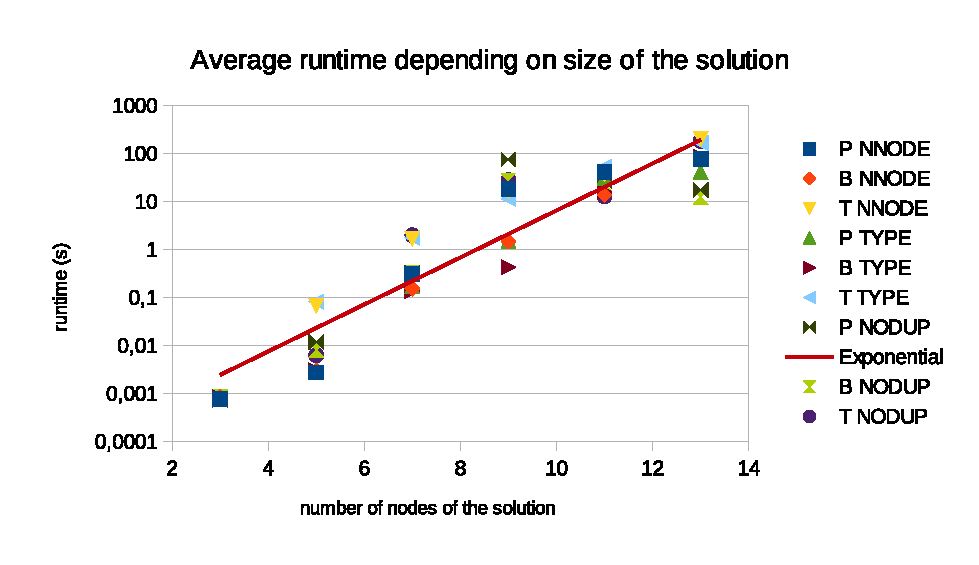
\includegraphics[width=0.95\textwidth]{time_vs_nof_nodes.eps}
    \caption{Average running time of the variants of the synthesis procedure depending on the number of nodes of the solution.}
    \label{fig:runtime_vs_nof_nodes}
\end{figure}
In the previous sections we mentioned a second factor: the size of the solution to be synthesised. Figure~\ref{fig:runtime_vs_nof_nodes} shows that the average running time for all nine variants of the synthesis procedure depends exponentially on the number of nodes of the solution found. This goes along with the intuition that a bigger program is more difficult to synthesise.

For example, if we have $n$ possibilities to generate a program consisting of one node, that is \lstinline!?x! where we have $n$ possibilities to instantiate the hole \lstinline!?x!, then we will have $n^2$ possibilities to generate a program with three nodes, that is \lstinline!?$x_1$ ?$x_2$! where we have $n$ possibilities to instantiate each hole.


\TODO{Delete this question or do something with it. We cannot answer it, we do not have enough data.}
More surprisingly, the individual results show that there must be some other factor influencing the runtime. Take, for example, \lstinline?enumFromTo?, \lstinline?stutter? and \lstinline?nth?. All three of them have a solution with exactly $13$ nodes, but their runtimes differ at least by an order of magnitude. What does make \lstinline?nth? generate in less than \SI{1}{s}, \lstinline?stutter? a hundred times slower and \lstinline?enumFromTo? to time out in most of the cases?

In our simple intuitive explanation of the exponential dependency of the synthesis time with the size of the solution we completely ignored the contribution of types to search space pruning.

\subsection{Cost functions}
Cost functions are an instrument to prioritize some programs over others and as such have an impact on the running time. We extensively evaluated three of the cost functions described in Section~\ref{Cost functions}: \textit{nof-nodes}, \textit{nof-nodes-simple-type} and \textit{no-same-component}. In the following we will see how they affect the runtime and which programs they prefer.

\begin{description}
\item[nof-nodes] prioritises shorter programs and prefers input variables to library components to holes. This means that the programs
\begin{lstlisting}[style=plain]
head [List Int -> List Int] (nil [List Int -> List Int]) ?xs
map Int Int succ ?xs
\end{lstlisting}
will have the same cost. It seems natural that paired with the \textsc{Plain} strategy it leads usually to higher running time than other cost functions.

\item[nof-nodes-simple-type] additionally penalises arrow types appearing in type applications. Its impact on the runtime is comparable to the introduction of pruning based on black lists.\TODO{Finish to write this section.\\} This preference leads to a larger solution for \lstinline!length!.
\end{description}


How cost functions influence the search space (\lstinline!(head (^26 -> ^27 -> Int) (nil (^26 -> ^27 -> Int))) ?2 ?3! has too complicated types appearing in the term, so it will have a higher cost in some of the cost functions. \lstinline!foldnat foldnat foldnat mul (mul 3 3) 3! takes a lot of time to evaluate, it will have a higher cost in no-same-component).

\begin{itemize}
\item Idea behind nof-nodes: smaller programs generalize better to the examples
\item Idea behind nof-nodes-simple-types: programs with smaller types are less "useless" (example with \lstinline?head nil?). Favor the use of input variables. But now a lot of "simple" but difficult to evaluate programs are synthesised, like the \lstinline?enumTo prod enumTo prod?.
\item Idea behind no-same-component: there are components that are usually used only once in a program, like \lstinline?foldr?, \lstinline?foldNat?. Another thing is that we penalize also complicated types of the form \lstinline?List (List (^5 -> List ^4))? that had no additional cost in nof-nodes-simple-types. But now types overweight the number of nodes and simple programs like \lstinline?foldr add zero _0? weight more than programs like \lstinline?add mul sub prod enumTo...?.
\item Idea behind no-same-component-bigger-constants: make all constants bigger so that we can differentiate more between the constants and so that nodes count more than types.
\item Idea behind no-same-component-even-bigger-constants: see above. (well, then you failed. your constants for types are pretty much as big as those for terms...). Why it's bad? See above.
\end{itemize}

\subsection{Examples}
Another factor that greatly impacts on performance is the choice and the number of provided input-output examples. As our procedure evaluates every closed program it synthesises on at least the first input-output example, we must make sure that the first input-output example is
\begin{enumerate}[a.]
\item small enough, so that also undesirable programs like \lstinline?enumTo (prod (enumTo (prod xs)))? do not get stuck or run out of memory trying to construct a list with $479001600$ elements, which happens already for the at first sight innocent input \lstinline?[2,2,3]?.
\item expressive enough to rule out many programs, so that there is no need to fall back on the other, often bigger, input-output examples.
\end{enumerate}
Clearly, using as few and as small input-output examples as possible has a positive effect on performance. On the other side, too few and too general input-output examples can lead to the synthesis of the wrong program, that is a program that satisfies all provided input-output examples but that does not generalise in the expected way. This was especially a problem with \lstinline?enumFromTo? and \lstinline?member?.
\TODO{Put a concrete example with enumFromTo}
\lstinline?con Int _0 (drop Int _0 )enumTo _1))? well, this is a real solution\\
\lstinline?filter Int (b_leq _0) (con Int b_zero (enumTo _1))?\\
On input \lstinline?enumFromTo 1 3 = [1,2,3]? and \lstinline?enumFromTo 2 4 = [2,3,4]? we get the program \lstinline?con Int _0 (con Int (b_succ _0) (con Int _1 (nil Int)))?

for (1,2) and (1,3) we get \lstinline?enumTo _1? or \lstinline?b_foldNatNat (List Int) (con Int) (nil Int) _1? depending on the components we give.

for (1,2) and (2,3) we get \lstinline?con Int _0 (con Int _1 (nil Int))?

for (1,2) and (2,4) we get \lstinline?con Int _0 (map Int Int (b_add _0) (enumTo _0))? 

\subsection{Blacklist}
\TODO{Make and insert mentioned figures: the manual black list\\}
The search space abounds of superfluous programs that are equivalent to smaller ones. In Section~\ref{Black list} we introduced a way to leverage this inconvenience: Pruning based on black lists. This approach allows us not to explore further programs that will surely lead to a solution bigger than the optimal one, like \lstinline!append [X] (nil [X]) ?$xs$!, or not lead to a solution at all, like \lstinline!(head [?$X_1$ -> ?$X_2$ -> $X_3$] (nil [?$X_1$ -> ?$X_2$ -> $X_3$])) ?$x_1$ ?$x_2$!.

A longer black list allows to prune more superfluous programs and sinks considerably the number of programs our synthesis procedure needs to consider before finding a solution. However, black list pruning is extremely expensive in our implementation. Each element of the black list is matched against every subtree of every program with holes that is generated. That is, there is a trade-off between the length of the black list and the gain in performance that we can get.

Figure~\ref{fig:manual_blacklist} shows the black list  we used to evaluate the benchmarks. We manually compiled it combining unwanted patterns often seen in the search space with some carefully chosen automatically generated identity functions. We also added some extremely increasing functions like \lstinline!foldNat [Int] (foldNat [Int] (mul n) 1) 1 m! that represented a problem for our evaluator.
\TODO{If you have time, try to figure out what mathematical function it corresponds to}.

In Table~\ref{fig:table_with_runtimes} we see that the runtime profits the most from the introducing of black list pruning when we use the cost function \textit{nof-nodes}.
The running time drops less significantly if we use other cost functions. A possible explanation of this behaviour could be the fact that other cost functions give a higher cost to those programs that are filtered with our black list.

We could also empirically see that pruning using black lists is very helpful in the presence of "useless" functions that increase the branching factor, for example \lstinline?flip?, \lstinline?const? or \lstinline?uncurry?. Forbidding a fully applied \lstinline?flip?, \lstinline?const? or \lstinline?uncurry? has a comparable effect on performance to taking those components out of the library. However, since we are not taking those components out of the library, we are still able to synthesis functions that need them.

\subsection{Templates}
\TODO{Write this\\}
Explain why templates perform so poorly (hm... because they don't do BFS, that is they have to explore every branch to the "end"?)

Maybe show "strange" solutions? But we already have them in the section about solutions.

\note{Short section explaining that the templates you generate are not the templates you expect and why}
I found one example, where templates help! For \lstinline?dropmax? I had a run out of memory exception with plain enumeration and I could synthesise it in 7 seconds with templates!
(Ok, I modified templates to put in only really higher-order components and close every hole, no matter the type). More resistant to the choice of examples.

\subsection{Stack vs Queue expansion}
As already mentioned in Section~\ref{Search space}, we have two open questions in our best first search:
\begin{enumerate}[a.]
\item what program to expand next
\item which hole of this program to expand first
\end{enumerate}
In the previous section we addressed the first question with different cost functions. In this section we focus on the second one.

Among all possible heuristics to determine which hole of the least-cost program to expand next, we chose to discuss two. In the first one the open holes of a program are organised in a stack, as opposed to the second one, where the open holes are kept in a queue.

Organising the open holes of a program into a stack leads to the expansion of the holes from left to right. To give some intuition we provide a derivation of \lstinline?mapAdd? featuring the stack of open holes on the right of the program, where \lstinline?xs? represents the input list and \lstinline?n? the amount of the increment.
\begin{lstlisting}[style=plain]
(?$x_0$, [$x_0$]) $\longrightarrow$
(?$x_1$ ?$x_2$, [?$x_1$, ?$x_2$]) $\longrightarrow$
(?$x_3$ ?$x_4$ ?$x_2$, [?$x_3$, ?$x_4$, ?$x_2$])) $\longrightarrow$
(map [Int] ?$x_4$ ?$x_2$, [?$x_4$, ?$x_2$]) $\longrightarrow$
(map [Int] (?$x_5$ ?$x_6$) ?$x_2$, [?$x_5$, ?$x_6$, ?$x_2$]) $\longrightarrow$
(map [Int] (add ?$x_6$) ?$x_2$, [?$x_6$, ?$x_2$]) $\longrightarrow$
(map [Int] (add n) ?$x_2$, [?$x_2$]) $\longrightarrow$
(map [Int] (add n) xs, [])
\end{lstlisting}
Left-to-right expansion often lead to faster synthesis, because leftmost holes have usually more constraints on their type. Consider the program \lstinline!?$x_3$ ?$x_4$ ?$x_2$! from the derivation of \lstinline??. We know more about \lstinline!?$x_3$! than about \lstinline!?$x_2$!: The first one must be a function that takes two arguments of some type and returns a list of integers, whereas the second hole could be anything. Furthermore, the instantiation of \lstinline!?$x_3$! with \lstinline?map [Int]? imposes some constraints on the types of \lstinline!?$x_4$! and \lstinline!?$x_2$!.

Keeping the open holes of a program in a queue leads to the expansion of the hole with the smallest depth first. This could be useful to control the depth of a program, but in practice it has a substantial drawback. Consider again the derivation of \lstinline?mapAdd?. The first three steps are the same, but in the program \lstinline!?$x_3$ ?$x_4$ ?$x_2$! we would now try to expand the hole \lstinline!?$x_2$!, that we have absolutely no information about. Every library component and every input variable are valid instantiations of this hole. Thus, this expanding strategy leads to a higher branching factor and explores many useless programs like \lstinline!?$x_3$ ?$x_4$ map! and \lstinline!map (?$x_5$ foldr) xs!.

We used the stack-based expansion strategy throughout all runtime evaluations of the benchmarks.

\section{Synthesised solutions}
\TODO{Rewrite programs in normal style and put listing blocks with programs instead of inlining everything\\}
Most of the synthesised solutions are precisely the ones we would have written by hand. Interestingly, for some programs different variants of the synthesis procedure find two different valid programs of the same size. For example, for \lstinline?replicate? we find following two solutions.
\begin{lstlisting}
replicate [X] n x
    = map Int [X] (const [X] Int x) (enumTo n)
    = foldNat (List X) (con [X] x) (nil [X]) n
\end{lstlisting}


Sometimes, as for example for \lstinline?length?, two solutions of different sizes are found.
\begin{lstlisting}
length [X] xs
    = foldr [X] [Int] (const [Int -> Int] [X] succ) zero xs
    = sum (map [X] [Int] (const [Int] [X] (succ zero)) xs)
\end{lstlisting}
 The reason is that the cost function \textit{nof-nodes-simple-type} assigns a higher cost to the first solution, as it contains an arrow type.

For the few benchmarks that can use \lstinline?foldl? and \lstinline?foldr? interchangeably, like \lstinline?concat?, \lstinline?maximum? and \lstinline?sum?, different variants find different programs. The different variants of the synthesis procedure do not show clear preference for the one or the other. They can use \lstinline?foldr? for one of such programs and \lstinline?foldl? for the other.

Interesting is the case of \lstinline?multfirst? and \lstinline?multlast?, where following two solutions are found.
\begin{lstlisting}
multfirst [X] xs
    = map [X] [X] (const [X] [X] (head [X] xs)) xs
    = replicate [X] (length [X] xs) (head [X] xs)
\end{lstlisting}
We omit the analogous solutions for \lstinline!multlast! for brevity.
The different synthesis procedures show a clear preference for the one or the other. For example, all synthesis procedures using the \textsc{Template} exploration strategy seem to prefer the use of the higher-order \lstinline?map? to the first-order \lstinline?replicate?. This has to do with the depth of the first-order search. The search from a particular template (in this case the template with no higher-order functions) times out before reaching programs with three components. On the other hand, the search starting from the template \lstinline!map [?Y] [X] (const [?Y] [X] ?$x_1$) ?$x_2$! succeeds within the timeout.

The preference of the \textsc{Template} exploration strategy for solutions containing higher-order functions leads to unexpectedly large programs. For example, one of the solutions for \lstinline?factorial? is
\begin{lstlisting}
factorial n
    = prod (foldr [List Int] [List Int]
        (foldl [List Int] [Int] (const [List Int] [Int]))
        (enumTo n)
        (nil [List Int]))
\end{lstlisting}
instead of the much simpler \lstinline?prod (enumTo n)?. Note that since we are folding over an empty list, the two programs are completely equivalent.

There is a tendency to represent the constant integer $1$ as \lstinline?prod (nil [Int])? instead of \lstinline?succ zero?. And even if we forbid with a black list the patterns
\begin{lstlisting}
enumFromTo (succ zero) _
prod nil
\end{lstlisting}
the synthesis procedure with the \textsc{BlackList} exploration strategy still finds a way to express \lstinline?enumTo? using \lstinline?enumFromTo?: It simply falls back to 
\begin{lstlisting}
enumTo n
    = enumFromTo (div n n) n.
\end{lstlisting}
Of course, if we take the component \lstinline?enumFromTo? out of the library we can generate the desired program
\begin{lstlisting}
enumTo n
    = foldNatNat [List Int] (con [Int]) (nil [Int]) n.
\end{lstlisting}

Small programs are not always efficient. For example, for \lstinline?enumFromTo? we find the solution
\begin{lstlisting}
enumFromTo m n
    = con [Int] m (foldNat [List Int] (tail [Int]) (enumTo n) m)
\end{lstlisting}
that corresponds to generating a list from $1$ to the second input and then dropping the first part of the list. The more efficient solution
\begin{lstlisting}
enumFromTo m n
    = con [Int] m (map [Int] [Int] (add m) (enumTo (sub n m)))
\end{lstlisting}
is larger and thus it is generated only if we take \lstinline?foldNat? out of the library.

Sometimes the solution found by the synthesiser suggested other benchmarks we could try to synthesise. For example, after examining the aforementioned solution for \lstinline?enumFromTo? we realized that \lstinline?drop? can be implemented as
\begin{lstlisting}
drop [X] n xs
    = foldNat [List X] (tail [X]) xs n
\end{lstlisting}
Analogously, a "wrong" solution for \lstinline?member? turned out to be a clever implementation of \lstinline?isEven?, namely \lstinline?foldNat not true n?. Folding over an integer is similar to recursion over that integer. In this case the base case of the recursion is \lstinline?true? and in the inductive case we negate \lstinline?isEven (n-1)?.\\
Another unexpectedly clever solution is due to the absence of a polymorphic equality function. We only had equality over integers, thus the benchmark \lstinline?member? is not polymorphic but has the type \lstinline?Int -> List Int -> Bool?. This allowed the synthesiser to generate, along with the expected solution
\begin{lstlisting}
member n xs
    = not (is_nil [Int] (filter [Int] (eq n) xs)),
\end{lstlisting}
a special version that makes use of the fact that the product of a list is $0$ if the list contains at least one $0$ and that two numbers are equal if their difference is $0$.
\begin{lstlisting}
member n xs
    = is_zero (prod (map [Int] [Int] (sub n) xs))

\end{lstlisting}
This works in our implementation because our built-in integers can have negative values.

\section{Automatic black list}\label{Automatic black list}
We were able to automatically synthesise $300$ programs corresponding to the identity function for three different types using automatically generated input-output examples in under \SI{2}{s}. Because of their incremental nature, we need $8$ automatically synthesised input-output examples as opposed to the $2$-$3$ manual ones that would have been enough. Below that number there is no list of lists of integers that contains something but \lstinline?nil? or no list of length two. This implies that synthesis using automatically synthesised input-output examples is slower than synthesis using manual ones.

For the evaluation of the benchmarks we preferred compiling a manual black list mainly because of three reasons: 
\begin{enumerate}
\item All programs in the automatically generated black list correspond to the identity function.
\item Many automatically generated black list programs are unnecessary. For example, \lstinline?append (append nil nil) _? and \lstinline?concat (append nil _)? are not needed if the black list already contains \lstinline?append nil _?.
\item The automatically generated programs are all closed programs and as such they are too concrete. For example, instead of \lstinline?foldNatNat max _ zero?, \lstinline?foldNatNat const _ zero? and \lstinline?foldNatNat drop _ zero? we could just have the one program \lstinline?foldNatNat _ _ zero? that generalises all the programs with the idea that folding over the integer $0$ is the same as taking the initial value, no matter which function is used for folding.
\end{enumerate}

The first two points can be addressed with small modifications to the experimental set up: generate \lstinline?nil?, \lstinline?zero?, \lstinline?undefined? and other constants as well for the first and prune the black list after or during generation for the second.
The third point is way more complex. Partial evaluation of programs with holes could help to some extent, but at the end it is about the ability to abstract and generalise over programs.

\section{Comparison to related work}
\TODO{Put the table in LaTeX\\}
\TODO{Write this}
Comparison to Feser, to Nadia, to Escher and to Myth. Say that you cannot really compare the numbers because they weren't run on the same machine. Say the thing with the size of the specification and the number of components. Say you have components capturing (tail?) recursive behaviour (fold over lists and fold over integers).


%%% Local Variables:
%%% mode: latex
%%% TeX-master: "thesis"
%%% End:
